% \documentclass[10pt,a4paper]{article}
\documentclass[UTF8]{ctexart}
\usepackage{geometry}
\usepackage[utf8]{inputenc}
\usepackage{CJKutf8}
\usepackage{graphicx}
\usepackage{epsfig}
\usepackage{mathptmx}
\usepackage{times}
\usepackage{amsmath}
\usepackage{amssymb}
\usepackage{cite}
\usepackage{subfigure}
\usepackage{subfig}
\usepackage{verbatim}
\usepackage{multirow}
\usepackage{bm}
\usepackage{float}
\usepackage{etoolbox,xstring,mfirstuc,textcase}
\usepackage{indentfirst}
\usepackage{enumerate}
\author{沈艳晴}
\title{Assignment2--光流估计}
\geometry{left=3.18cm, right=3.18cm, top=2.54cm, bottom=2.54cm}

\begin{document}
\begin{CJK*}{UTF8}{gbsn}
\CJKindent%中文缩进专用
\maketitle


\begin{abstract}
从前两章节的运动场我们了解到,如果我们能够获取图像之间的运动场,进而我们便可以得到对应的三维物体的运动情况。
但在实际情况中,运动场并不容易得到。为了获取图像中点的运动,我们通过计算光流来近似真实的图像间运动。光流场本身存在不唯一性,且与运动场不完全一致,但在实际应用中仍然使用这种方法居多。
光流是图像亮度模式的表观运动,评估了两幅图像之间的变形。
\end{abstract}

\section{光流原理}\label{sec1}
\begin{figure}[htbp]
    \centering
    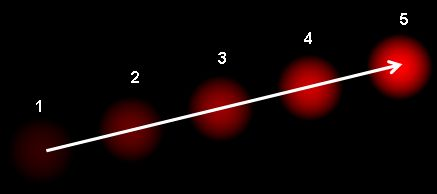
\includegraphics[height=4.5cm,width=8.5cm]{optical_flow_basic1.jpg}
    \caption{光流简化示意图}
    \label{fig:opti1}
\end{figure}
光流计算是基于物体运动的光学特性,因此有两个基本假设:
\begin{itemize}
    \item 运动物体的灰度在很短的时间间隔内保持不变
    \item 两帧图像之间像素点的运动微小
\end{itemize}
基于亮度不变的假设,我们可以得到基本的光流约束公式:
\begin{equation}
    I(x,y,t) = I(x+u(x,y),y+v(x,y),t+1)
\end{equation}
同时根据运动微小,我们在$(x,y)$处用泰勒级数线性展开,得到:
\begin{equation}
    I_{x} u + I_{y} v +I_{t} =0
\end{equation}
从上述公式中可以看出,在已知两幅图像的前提下,图像中的任何一个点对应都两个未知运动参数,而只有一个方程,约束不足。
\section{光流算法}

\subsection{Lucas-Kanade光流算法}\label{LK}
为了解决上节中提到的问题,LK光流算法在两个基本假设的基础上提出了另一个假设,即\textbf{邻域内运动具有空间一致性}(特例:物体边界等)。
基于这个假设,我们将一个方程两个未知数的问题转换成了多个方程两个未知数的问题。
表示如下:
\begin{equation}\left\{
    \begin{aligned}
        &I_{1x}u+I_{1y}v=-I_{1t}\\
        &I_{2x}u+I_{2y}v=-I_{2t}\\
        &...\\
        &I_{nx}u+I_{ny}v=-I_{nt}
    \end{aligned}\right.
\end{equation}
使用线性批处理最小二乘求解即可。
\begin{equation}
    \begin{bmatrix}u \\v \end{bmatrix} = 
        {\begin{bmatrix}
            \sum_{i=1}^{n}I_{ix}^2 & \sum_{i=1}^{n}{I_{ix} I_{iy}}\\
            \sum_{i=1}^{n}{I_{ix} I_{iy}} & \sum_{i=1}^{n}I_{iy}^2
        \end{bmatrix}}^{-1}
        \begin{bmatrix}
            -\sum_{i=1}^{n}{I_{ix}I_{t}} \\
            -\sum_{i=1}^{n}{I_{iy}I_{t}}
        \end{bmatrix}
\end{equation}
即,LK光流法是一种稀疏光流算法,并假设光流在像素点局部邻域是一个常数,然后使用最小二乘法对邻域中的所有像素点求解基本光流方程,从而计算时刻$t$到时刻$t+1$图像上每个像素点的平移运动情况。

\subsection{Horn-Schunck算法}
H-S法倾向于认为图像间的运动平滑,即就是让图像中的运动扭曲最小化,给出最平滑的结果。于是光流估计问题可以转化为如下全局扭曲能量的最小化问题:
\begin{equation}
    E = \iint \left[(I_{x} u + I_{y}v +I_{t})^{2} +\alpha^{2}(\lVert\nabla u \rVert ^ {2} + \lVert \nabla v \rVert ^ {2})\right] {{{\rm{d}}} x {{\rm {d}}} y}
\end{equation}
其中$I_x,I_y,I_t$是图像灰度在$x,y$和时间上的梯度,通过求解多维拉格朗日方程可以最小化该函数,即就是使			
$$
\begin{aligned}
    &{\frac {\partial L} {\partial u}}  -  {\frac {\partial} {\partial x}} {\frac {\partial L} {\partial u_{x}}}  -  {\frac { \partial} {\partial y}} {\frac {\partial L} {\partial u_ {y}}} = 0\\
    &{\frac {\partial L} {\partial v}}  -  {\frac {\partial} {\partial x}} {\frac {\partial L} {\partial v_ {x}}}  -  {\frac { \partial} {\partial y}} {\frac {\partial L} {\partial v_ {y}}} = 0
\end{aligned}
$$
其中L为全局扭曲能量的积分。

\subsection{基于金字塔的LK光流法}
章节~\ref{sec1}和~\ref{LK}中提到,假定运动微小,考虑两帧之间的物体位移可能很大,即运动快速,算法会存在较大的误差。为了解决这一问题,我们通过缩小像素尺寸在等价达到缩小物体“位移”的目的。
利用金字塔分层的方式,将原图像逐层分解,简单来讲即,上层金字塔具有低分辨率,其中的一个像素可以代表下一层的多个像素。利用这样的金字塔结构,\textbf{自上而下逐步由粗到细}修正运动估计。

具体步骤如下:
\begin{enumerate}
    \item 对每一帧图像建立一个高斯金字塔(高斯低通滤波+抽样)
    \item 选取图像的特征点,比如Shi-Tomasi角点等。特征选择的好,矩阵计算越有利。
    \item 针对某个具体点,从顶层开始估计光流变化。两帧图像的顶层光流初始估计设为$(0,0)$
    \item 每一层的光流估计分为初始估计和光流残差:初始估计可以由上一层的准确光流估计给出;光流残差则通过最小二乘迭代计算至前后两次计算偏差小于一定范围
\end{enumerate}
\section{视频跟踪中存在的问题及解决思路}

首先,我们上面介绍的方法在两帧图像之间使用效果并不总是那么好,通过最小化邻域范围内的匹配误差找到的下一帧的对应位置,并不一定准确;

其次,即使两帧之间追踪效果很好,但对于一个长视频来说,总共包含几百、几千帧的图像,第一帧图像的特征点会很快丢失,也会不断增加新的特征点,因此我们需要对特征点的丢弃、新增进行设计。

因此,在实际完成这个项目时,除了对金字塔LK光流算法进行实现外,还运用了一些技巧,保证光流估计的长期性和准确性。
\begin{itemize}
    \item 根据上一帧图像选取的特征点,得到下一帧对应点之后,再用对应点位置去回溯上一帧中的对应位置,通过比较原本的位置和回溯的位置,如果偏差大于一定范围便认为跟踪错误,进行丢弃。
    \item 每隔10帧,对特征点进行扩充
    \item 特征点的存储结构需要同时考虑时间和空间,每一帧图像都对应了一些二维坐标,同时对于这些坐标,每个坐标都有自己的变化过程。
\end{itemize}

\section{结果展示}
先对一帧图像进行特征点提取

然后通过光流估计法,在下一帧相邻图像中,在距离阈值范围内,寻找可靠临近点,并逐步更新特征角点位置,最后通过选取跟踪成功的点,估计物体在视频流中的运动轨迹


\end{CJK*}
\end{document}